\section{实验要求与实验目的}

\subsection{实验要求}
根据实验指导书，实验一的要求如下：
\begin{enumerate}
  \item 利用 AT89C51 微控制器的 P0 口作开关量输入口，P1 口作开关量输出口。
  \item 当 P0.x 端开关闭合时，对应 P1.x 口的 LED 发光二极管点亮；当 P0.x 端开关断开时，对应 P1.x 口的 LED 发光二极管熄灭。
  \item 画出 AT89C51 实现上述功能的完整电路图，包括微控制器电源、复位电路、晶振电路和控制电路。
  \item 完成全部程序和电路调试工作。
\end{enumerate}

\subsection{实验目的}
\begin{enumerate}
  \item 掌握 AT89C51 微控制器最基本电路的设计方法。
  \item 了解微控制器 I/O 端口的使用方法。
\end{enumerate}

\subsection{设计提示}
P0 口作为 I/O 使用时，需要配置上拉电阻，避免端口悬空导致读值不稳定。

\section{Proteus 原理图与硬件设计说明}

\subsection{原理图截图}
\begin{figure}[H]
  \centering
  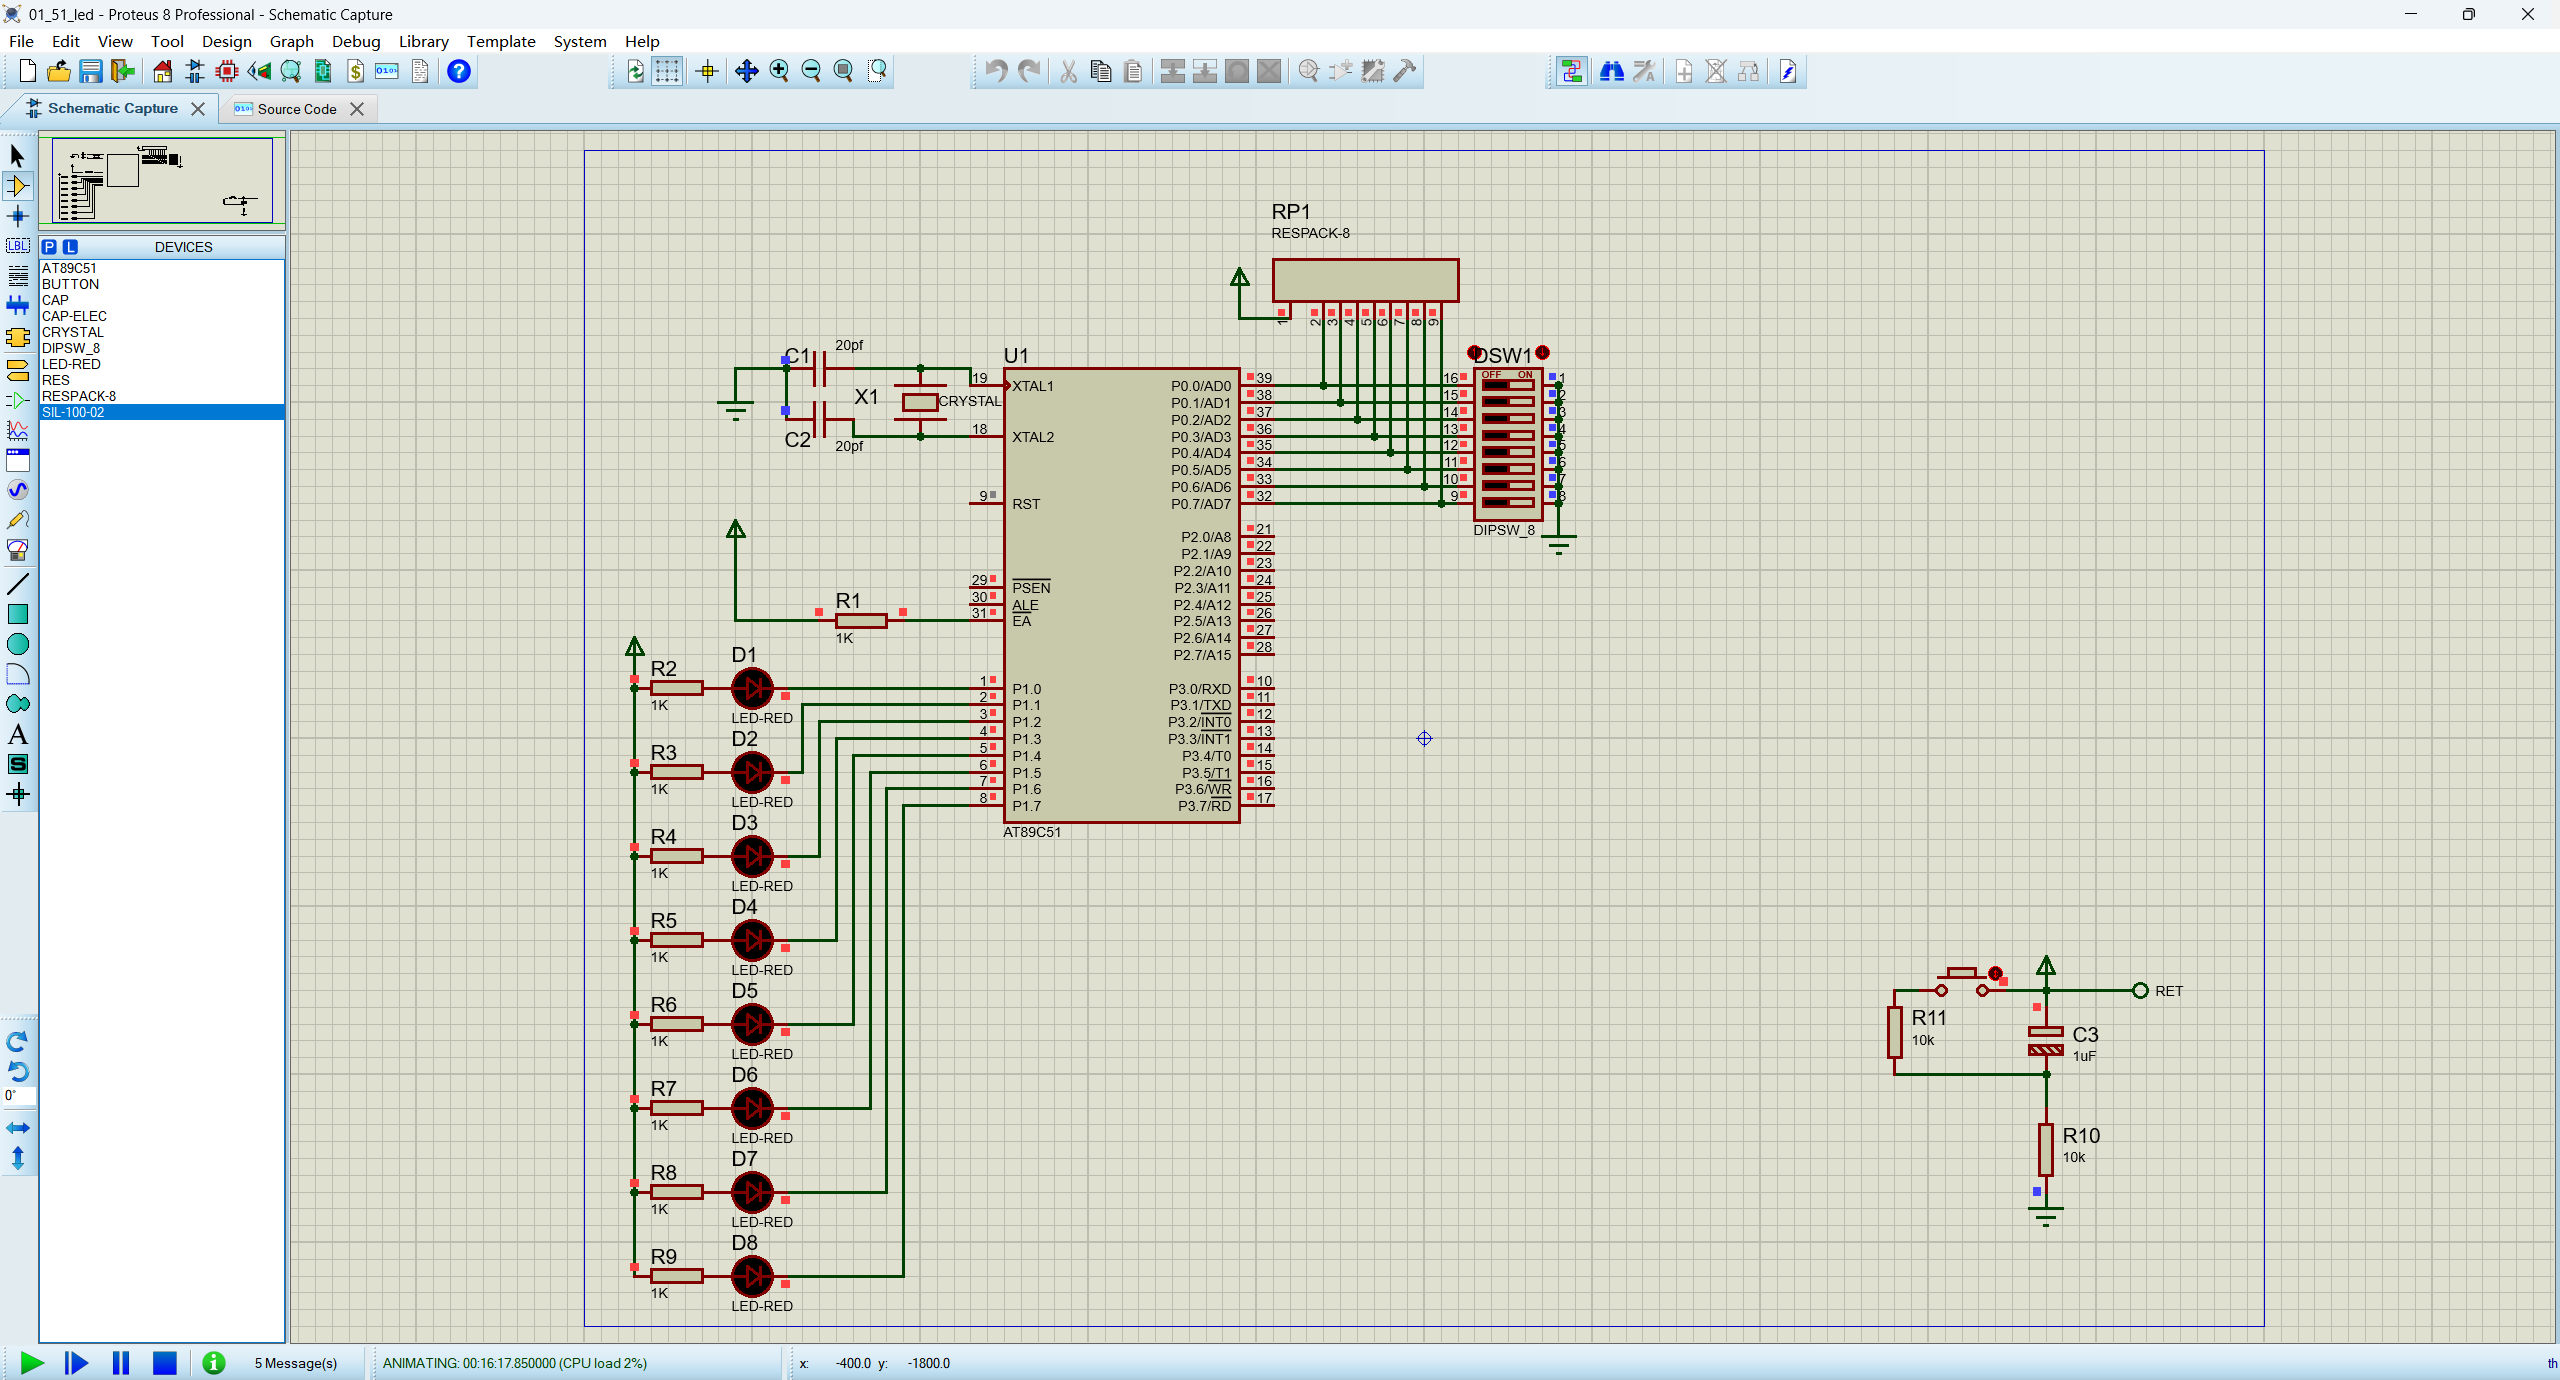
\includegraphics[width=0.95\textwidth]{images/ProteusSchematic.PNG}
  \caption{实验一 Proteus 原理图截图}
\end{figure}

\subsection{电路组成与功能对应关系}
本实验硬件电路由四个部分组成：
\begin{itemize}
  \item 电源与基础引脚：为 AT89C51 提供稳定工作电源，并完成必要控制引脚配置。
  \item 复位电路：保证上电时单片机进入确定初始状态，程序从复位入口开始执行。
  \item 晶振电路：由晶振和电容构成时钟网络，为 CPU 提供系统时钟。
  \item I/O 控制电路：P0 连接拨码开关输入，P1 连接 LED 输出，完成开关状态到灯状态的位对应映射。
\end{itemize}

结合原理图可见：
\begin{enumerate}
  \item SW1（DIPSW\_8）提供 8 位开关量输入；
  \item P0.0--P0.7 接收上述输入信号；
  \item P1.0--P1.7 分别驱动 D1--D8；
  \item 每个 LED 串联电阻，起限流与保护作用。
\end{enumerate}

\subsection{主要元件清单}
\begin{table}[H]
  \centering
  \caption{实验主要元件与模型}
  \renewcommand{\arraystretch}{1.35}
  \begin{tabular}{cllll}
    \toprule
    序号 & 元件名称 & 元件规格 & 所在元件库 & 工具模型 \\
    \midrule
    1 & 微控制器 & AT89C51 & Microprocessor & Component mode \\
    2 & 按钮/开关 & BUTTON & Switches \& Relay & Component mode \\
    3 & 晶振 & CRYSTAL & Miscellaneous & Component mode \\
    4 & 发光二极管 & LED-RED & Optoelectronics & Component mode \\
    5 & 电容 & CAP / CAP-ELEC & Capacitors & Component mode \\
    6 & 电阻 & RES & Resistors & Component mode \\
    7 & 拨码开关 & DIPSW\_8 & Switches \& Relay & Component mode \\
    8 & 电源与地 & POWER / GROUND & Terminals & Terminals mode \\
    9 & 电源输入端 & SIL-100-02 & Connectors & Component mode \\
    \bottomrule
  \end{tabular}
\end{table}

\section{软件设计与流程分析}

\subsection{程序流程图}
\begin{figure}[H]
\centering
\begin{tikzpicture}[
  node distance=10mm and 14mm,
  proc/.style={rectangle,rounded corners,draw=themecolor,fill=blue!3,minimum width=4.8cm,minimum height=9mm,align=center},
  io/.style={trapezium,trapezium left angle=75,trapezium right angle=105,draw=themecolor,fill=cyan!6,minimum width=5.2cm,minimum height=9mm,align=center},
  line/.style={-Latex,thick,draw=themecolor}
]
  \node[proc] (start) {程序开始};
  \node[proc,below=of start] (init) {初始化：\texttt{MOV P0, \#0FFH}};
  \node[io,below=of init] (readin) {读取输入：\texttt{MOV A, P0}};
  \node[io,below=of readin] (output) {输出结果：\texttt{MOV P1, A}};
  \node[proc,below=of output] (jump) {循环跳转：\texttt{SJMP LOOP}};

  \draw[line] (start) -- (init);
  \draw[line] (init) -- (readin);
  \draw[line] (readin) -- (output);
  \draw[line] (output) -- (jump);
  \draw[line] (jump.east) -| ++(1.6,0) |- (readin.east);
\end{tikzpicture}
\caption{实验一程序流程图}
\end{figure}

\subsection{完整实验代码}
\lstset{style=a51style}
\lstinputlisting[caption={01\_single\_led.A51 完整源码}]{code/01_single_led.A51}

\subsection{关键代码逐段说明}
\begin{table}[H]
  \centering
  \caption{关键指令功能说明}
  \renewcommand{\arraystretch}{1.35}
  \begin{tabular}{p{0.26\textwidth}p{0.68\textwidth}}
    \toprule
    指令或语句 & 作用说明 \\
    \midrule
    \texttt{ORG 0000H} + \texttt{LJMP MAIN} & 定义复位入口，单片机上电后从 0000H 跳转到主程序地址。 \\
    \texttt{ORG 0030H} & 主程序起始地址定义，便于与中断向量区域区分。 \\
    \texttt{MOV P0, \#0FFH} & 将 P0 各位写 1，使端口处于读取外部开关状态的工作方式。 \\
    \texttt{MOV A, P0} & 将 P0 当前 8 位输入状态读入累加器 A。 \\
    \texttt{MOV P1, A} & 将输入值直接输出到 P1，实现 8 位一一对应控制。 \\
    \texttt{SJMP LOOP} & 构成无限循环，实现实时轮询与实时响应。 \\
    \bottomrule
  \end{tabular}
\end{table}

\section{调试过程与实验结果}

\subsection{调试过程记录}
\begin{enumerate}
  \item 在 Keil 中编译 \texttt{01\_single\_led.A51}，确认语法与目标文件生成正常。
  \item 在 Proteus 中连接 AT89C51、拨码开关、LED、晶振、复位和供电电路。
  \item 加载编译生成程序，启动仿真。
  \item 逐位拨动 SW1，观察 D1--D8 是否按位同步变化。
  \item 对全灭、全亮、奇偶位组合等典型输入进行对照验证。
\end{enumerate}

\subsection{结果验证表}
\begin{table}[H]
  \centering
  \caption{输入输出对应关系验证}
  \renewcommand{\arraystretch}{1.35}
  \begin{tabular}{cccc}
    \toprule
    测试序号 & P0 输入（开关状态） & 预期 P1/LED 输出 & 结果 \\
    \midrule
    1 & 0x00 & 全灭 & 符合 \\
    2 & 0xFF & 全亮 & 符合 \\
    3 & 0x55 & 奇数位亮、偶数位灭 & 符合 \\
    4 & 0xAA & 偶数位亮、奇数位灭 & 符合 \\
    5 & 任意组合 & 位对位同步显示 & 符合 \\
    \bottomrule
  \end{tabular}
\end{table}

\subsection{编译信息}
从 A51 编译列表可确认：
\begin{itemize}
  \item 汇编器版本：A51 V8.2.7.0；
  \item 关键符号地址：\texttt{MAIN=0030H}，\texttt{LOOP=0030H}，\texttt{P0=0080H}，\texttt{P1=0090H}；
  \item 编译结果：\textbf{0 warning，0 error}。
\end{itemize}

\section{问题分析与改进建议}
\begin{enumerate}
  \item P0 口使用时应确认上拉网络有效，避免输入悬空导致 LED 状态抖动。
  \item 实际硬件中可加入按键消抖或软件延时，提高状态显示稳定性。
  \item 可扩展为中断方式采样，减少无效轮询占用。
\end{enumerate}

\section{实验结论}
本实验完成了基于 AT89C51 的开关量输入输出控制：P0 口读取开关状态，P1 口输出 LED 控制信号，最终实现输入与输出一一对应。通过本次实验，验证了单片机最基本电路（电源、复位、晶振、I/O 控制）与端口编程方法，达到实验指导书要求。

\appendix
\section{附录：编译清单摘要}
\lstset{style=a51style}
\lstinputlisting[caption={01\_single\_led.LST（节选）}]{code/01_single_led.LST}
